\documentclass[10pt]{jsarticle}
\usepackage{gaiyou}
\usepackage[dvipdfmx]{graphicx}
\usepackage[top=2cm, bottom=2cm, left=1.5cm, right=1.5cm]{geometry}

\begin{document}

\pagestyle{empty}

\setlength{\baselineskip}{13truept}

\title{植物自律化による自己育成システム}
\engtitle{Self-cultivation system by plant autonomization}
\supervisor{村松 聡}
\author{黒木 駿太}
\engsupervisor{Satoshi Muramatsu}
\engauthor{Shunta Kuroki}

\maketitle
\thispagestyle{empty}

\section{はじめに}
近年,植物の栽培方法は多様化しハウス栽培等に留まらず,屋内の植物工場で栽培される事例もある.
植物工場ではコンピュータ制御によって,水分や肥料,光や温湿度が植物にとって最適化される.
しかし,植物工場は建設の資金と時間を必要とすることや,栽培する植物は水耕栽培で採算性の良い品種の植物に限られてしまう.
また,最終的には人間が管理をしなければならない問題がある\cite{Paper01}.

一方,人間を始めとする動物は自発的に飲食や移動をを行い,自らの生命機能維持を他者に依存することなく最適な環境を獲得することができる.これらの特徴は動物のメリットである.
このことから,植物も動物のように能動的に生命機能維持の為の欲求を満たすことで,他者の助けなしに最適な環境を見つけ出し,効率的に生命活動を行うことが可能となる.

そこで本研究は人間による管理を必要としない,植物の能動的な行動で自己成長が行えるシステムの開発を行う.

\section{植物自律化}
植物自律化とは,能動的に行動できる植物を意味する.
具体的にはセンサにより自己状態を把握し,必要に応じてロボットで移動することを指す.
土壌の水分が減ると水分補給を行い,日差しが弱い場合にはより明るい場所を探すよう能動的に行動を行う.
それにより,動物のように自身の状態によって自由に行動し,他者に依存することのない生命活動を実現する.

\section{自動育成植木鉢ロボットシステム}
前章の植物自律化を実現するため,自動育成植木鉢ロボットシステムの製作を行った.
本システムではセンサ情報を元に作成された地図を用いてロボットの行動計画を行う.
地図情報は移動を行うごとに随時更新され,時間とともに情報の信頼性と予測精度が向上する.
Fig.\ref{robot_all}の本システムでは植物と環境センサを搭載し走行する自律移動ロボットと,水分を供給する給水ステーションで構成される.
\begin{figure}[ht]
    \centering
    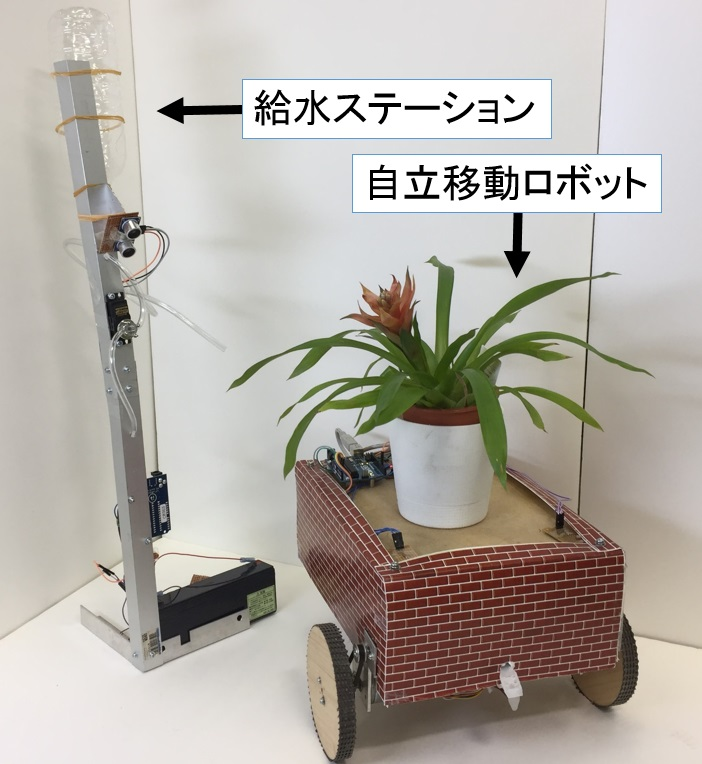
\includegraphics[width=0.25\textwidth]{img/IMG_3901a.JPG}
    \caption{ロボットシステム全体}
    \label{robot_all}
\end{figure}
\subsection{自律移動ロボット}
自律移動を行うためには植木鉢の搭載が可能な移動機構が必須となる.
狭い場所においても旋回が可能であり,制御が容易かつ製作コストが少ない対向2輪型の自律移動ロボットを製作した.
ロボットには環境情報を取得するセンサが搭載されており,センサ及びロボットの制御は小型コンピュータを中心として行っている.
また,ネットワークを介することで,他の機器との連携も可能である.
\subsubsection{ハードウェア}
%ロボットの仕様は表\ref{shiyou}となっている.
ロボットの筐体は安全性と管理の観点から2段に分かれている.下段にはモータや制御機器などの電装系,上段にはセンサ類と植木鉢を設置し,サイドカバーをつけることで水濡れによるショートやデザイン性の向上を図っている.
制御PCやセンサ類など,ロボットの構成はFig.\ref{robot_hard}のようになっている.
\begin{figure}[t]
    \centering
    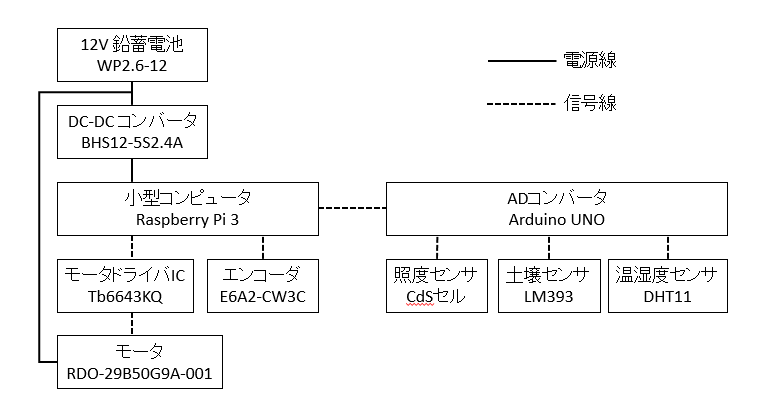
\includegraphics[width=0.5\textwidth]{img/hard.png}
    \caption{ロボット構成概要}
    \label{robot_hard}
\end{figure}
搭載しているセンサは3種類で,照度,温湿度,土壌水分である.なお,照度センサは四隅に搭載し植物の影の影響を軽減している.
%\begin{table}[t]
%    \begin{center}
%    \caption{自律移動ロボットの仕様}
%    \begin{tabular}{|c|l|} \hline
%        サイズ(WxHxD) & 230x205x300[mm] \\ \hline
%        重量 & 2.5[kg] \\ 
%        & (バッテリーを除く) \\ \hline
%        バッテリー & 鉛蓄電池 \\
%        & 容量 : 2.6Ah/31Wh \\
%        & 稼働時間 : 最大6時間以上 \\ \hline
%        センサ & ロータリーエンコーダ x 2 \\
%        & 照度センサ x 3 \\
%        & 温湿度センサ x 1 \\
%        & 土壌センサ x 1 \\ \hline
%        駆動部 & 減速機一体型DCモータ \\
%        & ホイール直付け \\ \hline
%        移動速度 & 最大4km/h \\ \hline
%        登坂能力 & 最大勾配1\% \\ \hline
%        積載重量 & 最大5[kg] \\ \hline
%        プラットフォーム & Ubuntu 16.04 for ARM \\ \hline
%    \end{tabular}
%    \label{shiyou}
%    \end{center}
%\end{table}

\subsubsection{ソフトウェア}
自律移動のためのソフトウェアの多くはRaspberry Pi上で動いており,センサで読み込んだ値を元にモータの制御を行っている.
まず,センサ情報は環境の世界座標と一緒に保存され,Fig.\ref{map}ようにグリットマップで管理される.グリットマップはセンサの種類ごとにレイヤー分けされる.
\begin{figure}[t]
    \centering
    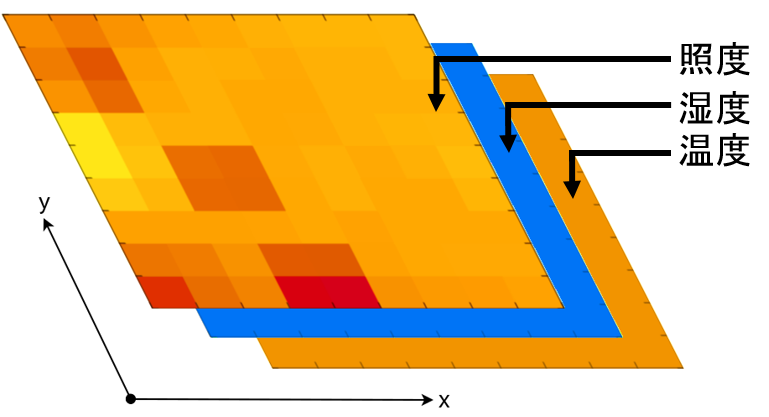
\includegraphics[width=0.4\textwidth]{img/map_setumei.png}
    \caption{多次元グリットマップ}
    \label{map}
\end{figure}
この地図を元に行動計画を行う.
土壌水分量が少ない場合は次節で説明する給水ステーションに向かい,照度や温度が低い場合には周囲を散策し最適な位置に移動を行う.
そのための自律移動はモータとエンコーダの組み合わせで行っている.
自己位置はオドメトリを用いて推定している.

\subsection{給水ステーション}
植物が自律的に成長するため水分の摂取は必須である.
水分を自発的に摂取するためにも,水を提供するロボットは必要なサービスである.
本ロボットは前章の自律移動ロボットとセットで利用される事を想定して作成た.距離センサを用いて近づいたものに水分を与えるものとなっている.
\subsubsection{ハードウェア}
フレームは軽く,錆びることのないアルミニウム製で,タンクは取り外しが可能となっている.
バルブの開閉機構にはRCサーボを利用し,制御のためにArduinoを用いている.
ロボットの接近を検知する距離センサは上部より下を見下ろすような形で設置し,誤検知を防いでいる.
また,ノズルの位置の調整を行うことで様々な植物に対応が可能となっている.
\subsubsection{ソフトウェア}
ロボットの制御にはArduino UNOを使用し,サーボモータと距離センサの組み合わせで動作する.
距離センサで本ロボットの前に接近したものを検知するとRCサーボを用いてバルブを回転させ給水し,一定時間水分を与えた後再びRCサーボでバルブを元の位置に戻すプログラムとなっている.

\section{実験}
\subsection{センサ情報に基づく環境地図の作成実験}
\label{sec_map}
本実験では温湿度センサ,照度センサに基づき環境情報をマッピングできているかを確認する.
2[m]x2[m]の環境を一辺0.2[m]のグリットで分割し,各グリットごとにセンサ情報を計測した.
計測したセンサ情報に基づいて,マッピングを行った.
マッピングの一例として照度センサの結果をFig.\ref{light_map}に示す.
Fig.\ref{light_map}は環境の明るさを10bit階調で計測し,その値をグリットのヒートマップとして表現したものである.
この結果より,センサ情報を環境の世界座標と関連付けてマッピングできている事を確認した.
\begin{figure}[t]
    \centering
    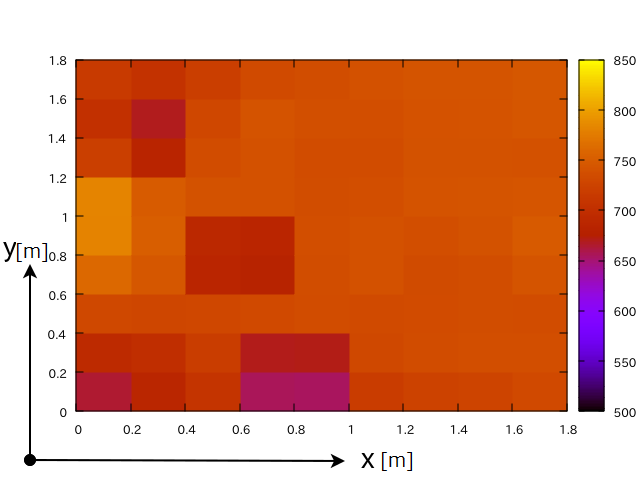
\includegraphics[width=0.3\textwidth]{img/light_xya.png}
    \caption{照度センサのグリットマップ}
    \label{light_map}
\end{figure}
\subsection{経路の追従実験}
\label{sec_keiro}
センサ情報 と環境地図の情報から計画された移動すべき経路に沿って追従可能であるか確認した.
実験環境は周長6[m]程のテーブル周辺で,行動計画で生成された経路と走行結果のズレを評価する.
結果をFig.\ref{tsuizyu}に示す.
実験結果より,1\%程度で行動計画にしたがって追従することを確認した.
\begin{figure}[t]
    \centering
    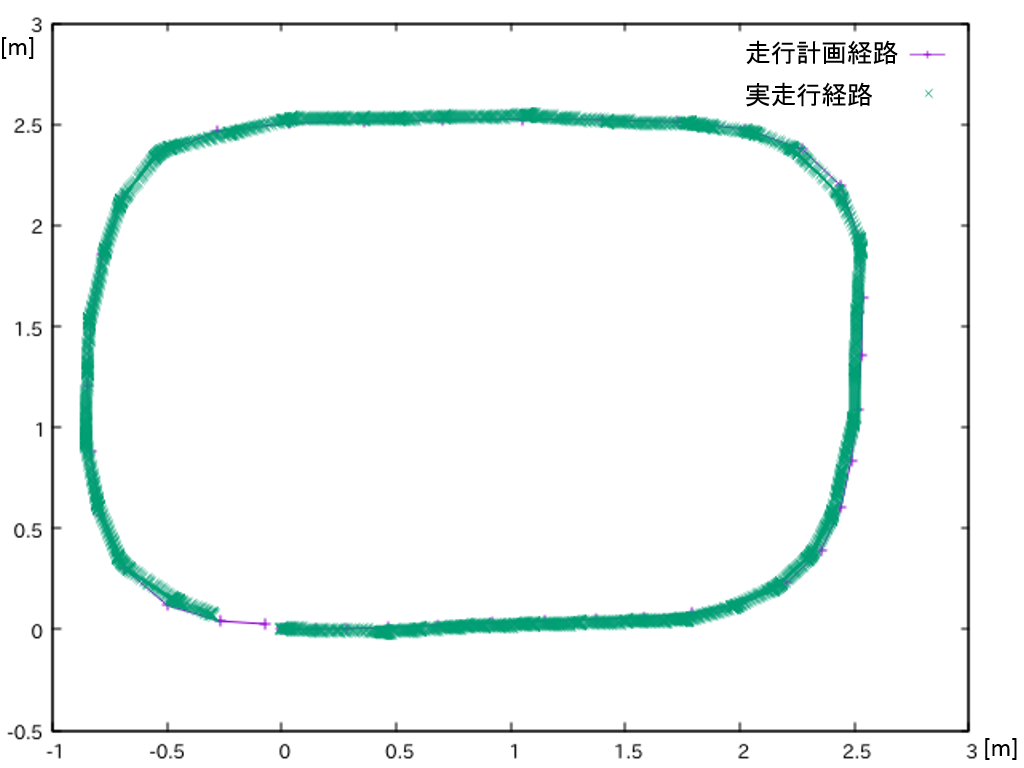
\includegraphics[width=0.4\textwidth]{img/tsuizyua.png}
    \caption{ロボットの誘導}
    \label{tsuizyu}
\end{figure}

\subsection{自己育成システムの実証}
\ref{sec_map}及び\ref{sec_keiro}より,植物がセンサ情報に基づき能動的に行動できるか確認した.
行動中の様子をFig\ref{mizu}に示す.
これは土壌水分センサの情報に基づき,給水ステーションと連携して植物が能動的に水分補給を行った様子である.
このことから本研究のシステムによって,植物が能動的に行動を行っていることを確認できた.
\begin{figure}[t]
    \centering
    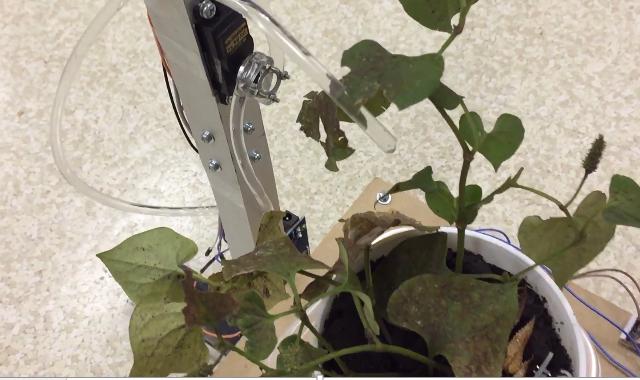
\includegraphics[width=0.3\textwidth]{img/mizu.png}
    \caption{水分補給の様子}
    \label{mizu}
\end{figure}

\section{おわりに}
本研究では植物の能動的な行動により自己育成を行うことを目的に,自律移動ロボットと給水ステーションを作成た.
それらを用いて環境のセンシングや自律移動を元に能動的な行動計画を行い,自己育成を行うことができた.

今後は台数を増やし植物同士のコミュニケーションなどの様子を確認する予定である.

\begin{thebibliography}{10}

%%参考文献
\bibitem{Paper01}
山下真人, 山本緑, 高橋真一, 溝田陽子, 末田香恵, 久保啓治: 植物工場の現状の課題とその一検証,
大林組技術部,{\bf 大林組技術研究報}-No.77, pp.001-006 (2013)
\end{thebibliography}

\end{document}
